\documentclass[twocolumn]{article}
\usepackage{tikz}
\usepackage{amsmath}
\usepackage[margin=0.5in]{geometry}

\begin{document}

% LaTeX Figure: Bidirectional Information Flow
% Top-Down (Feature Fusion) + Bottom-Up (Gradient Flow)

\begin{figure*}[t]
\centering
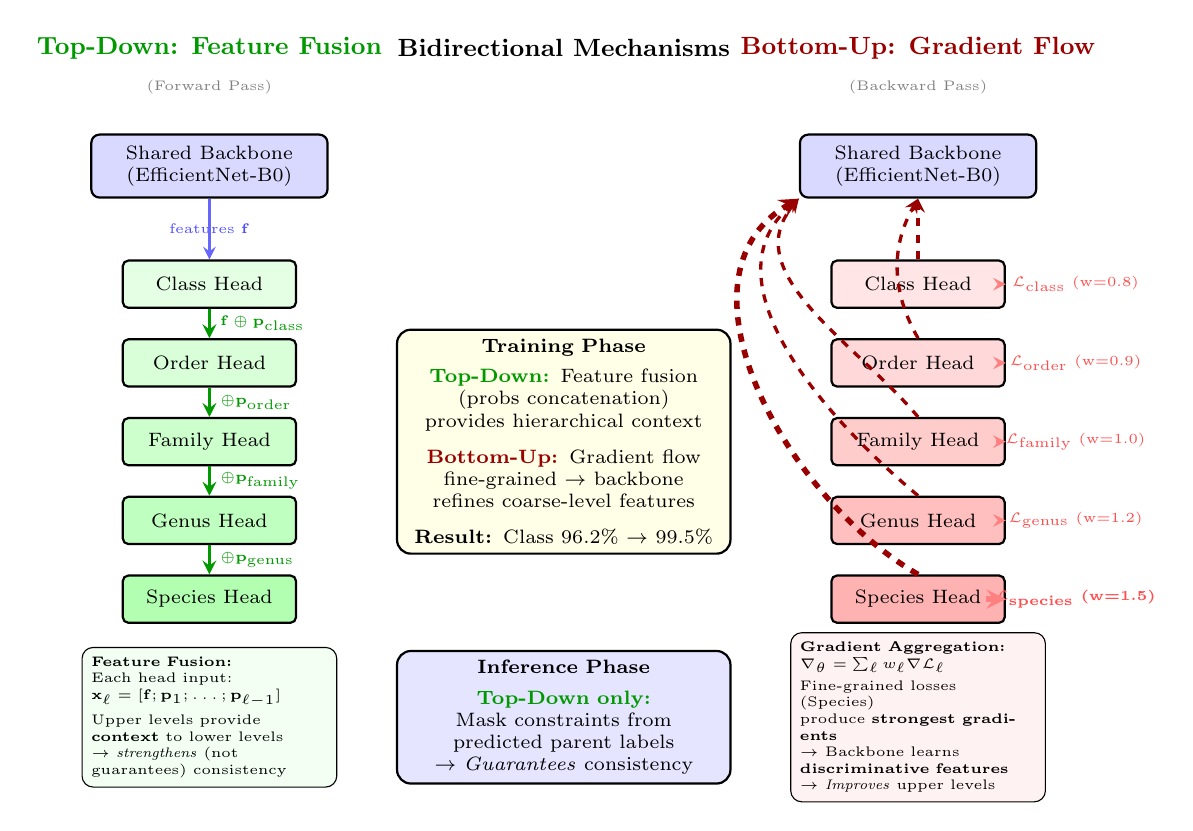
\begin{tikzpicture}[
    node distance=0.6cm and 1.5cm,
    box/.style={rectangle, draw, thick, minimum width=2.2cm, minimum height=0.6cm, align=center, font=\scriptsize},
    backbone/.style={box, fill=blue!15, rounded corners=3pt, minimum width=3cm, minimum height=0.8cm},
    head/.style={box, fill=gray!15, rounded corners=2pt},
    topdown/.style={->, >=stealth, thick, green!60!black, line width=1.2pt},
    bottomup/.style={->, >=stealth, thick, red!60!black, line width=1.2pt, dashed},
    feature/.style={->, >=stealth, thick, blue!60, line width=1pt},
    grad/.style={->, >=stealth, thick, red!50, line width=1pt, dashed},
    label/.style={font=\tiny, text=gray}
]

% ===== LEFT SIDE: TOP-DOWN (Forward Pass / Feature Fusion) =====
\node[font=\small\bfseries, text=green!60!black] at (-4.5, 5) {\textbf{Top-Down: Feature Fusion}};
\node[font=\tiny, text=gray] at (-4.5, 4.5) {(Forward Pass)};

% Backbone
\node[backbone] (l_backbone) at (-4.5, 3.5) {Shared Backbone\\(EfficientNet-B0)};

% Features arrow
\node[font=\tiny, text=blue!70] at (-4.5, 2.7) {features $\mathbf{f}$};

% Heads with probability flow
\node[head, fill=green!10] (l_class) at (-4.5, 2) {Class Head};
\node[head, fill=green!15] (l_order) at (-4.5, 1) {Order Head};
\node[head, fill=green!20] (l_family) at (-4.5, 0) {Family Head};
\node[head, fill=green!25] (l_genus) at (-4.5, -1) {Genus Head};
\node[head, fill=green!30] (l_species) at (-4.5, -2) {Species Head};

% Top-down arrows with labels
\draw[feature] (l_backbone) -- (l_class);
\draw[topdown] (l_class) -- (l_order) node[midway, right, font=\tiny, text=green!60!black] {$\mathbf{f} \oplus \mathbf{p}_{\text{class}}$};
\draw[topdown] (l_order) -- (l_family) node[midway, right, font=\tiny, text=green!60!black] {$\oplus \mathbf{p}_{\text{order}}$};
\draw[topdown] (l_family) -- (l_genus) node[midway, right, font=\tiny, text=green!60!black] {$\oplus \mathbf{p}_{\text{family}}$};
\draw[topdown] (l_genus) -- (l_species) node[midway, right, font=\tiny, text=green!60!black] {$\oplus \mathbf{p}_{\text{genus}}$};

% Annotation box
\node[draw, rounded corners, fill=green!5, font=\tiny, text width=3cm, align=left] at (-4.5, -3.5) {
\textbf{Feature Fusion:}\\
Each head input:\\
$\mathbf{x}_\ell = [\mathbf{f}; \mathbf{p}_1; \ldots; \mathbf{p}_{\ell-1}]$\\[2pt]
Upper levels provide\\
\textbf{context} to lower levels\\
$\rightarrow$ \textit{strengthens} (not\\
guarantees) consistency
};


% ===== RIGHT SIDE: BOTTOM-UP (Backward Pass / Gradient Flow) =====
\node[font=\small\bfseries, text=red!60!black] at (4.5, 5) {\textbf{Bottom-Up: Gradient Flow}};
\node[font=\tiny, text=gray] at (4.5, 4.5) {(Backward Pass)};

% Backbone
\node[backbone] (r_backbone) at (4.5, 3.5) {Shared Backbone\\(EfficientNet-B0)};

% Heads
\node[head, fill=red!10] (r_class) at (4.5, 2) {Class Head};
\node[head, fill=red!15] (r_order) at (4.5, 1) {Order Head};
\node[head, fill=red!20] (r_family) at (4.5, 0) {Family Head};
\node[head, fill=red!25] (r_genus) at (4.5, -1) {Genus Head};
\node[head, fill=red!30] (r_species) at (4.5, -2) {Species Head};

% Loss nodes on the right
\node[font=\tiny, text=red!70] (loss_c) at (6.5, 2) {$\mathcal{L}_{\text{class}}$ (w=0.8)};
\node[font=\tiny, text=red!70] (loss_o) at (6.5, 1) {$\mathcal{L}_{\text{order}}$ (w=0.9)};
\node[font=\tiny, text=red!70] (loss_f) at (6.5, 0) {$\mathcal{L}_{\text{family}}$ (w=1.0)};
\node[font=\tiny, text=red!70] (loss_g) at (6.5, -1) {$\mathcal{L}_{\text{genus}}$ (w=1.2)};
\node[font=\tiny, text=red!70, font=\tiny\bfseries] (loss_s) at (6.5, -2) {$\mathcal{L}_{\text{species}}$ (w=1.5)};

% Gradient arrows from losses to heads
\draw[grad] (loss_c) -- (r_class);
\draw[grad] (loss_o) -- (r_order);
\draw[grad] (loss_f) -- (r_family);
\draw[grad] (loss_g) -- (r_genus);
\draw[grad, line width=2pt] (loss_s) -- (r_species);

% Gradient convergence to backbone
\draw[bottomup] (r_class.north) -- (r_backbone.south);
\draw[bottomup] (r_order.north) to[out=120, in=-120] (r_backbone.south);
\draw[bottomup] (r_family.north) to[out=130, in=-130] (r_backbone.south west);
\draw[bottomup] (r_genus.north) to[out=140, in=-140] (r_backbone.south west);
\draw[bottomup, line width=2pt] (r_species.north) to[out=150, in=-150] (r_backbone.south west);

% Annotation box
\node[draw, rounded corners, fill=red!5, font=\tiny, text width=3cm, align=left] at (4.5, -3.5) {
\textbf{Gradient Aggregation:}\\
$\nabla_\theta = \sum_\ell w_\ell \nabla \mathcal{L}_\ell$\\[2pt]
Fine-grained losses (Species)\\
produce \textbf{strongest gradients}\\
$\rightarrow$ Backbone learns\\
\textbf{discriminative features}\\
$\rightarrow$ \textit{Improves} upper levels
};


% ===== CENTER: Summary =====
\node[font=\small\bfseries] at (0, 5) {\textbf{Bidirectional Mechanisms}};

% Central summary box
\node[draw, thick, rounded corners=5pt, fill=yellow!10, font=\scriptsize, text width=4cm, align=center] at (0, 0) {
\textbf{Training Phase}\\[3pt]
\textcolor{green!60!black}{\textbf{Top-Down:}} Feature fusion\\
(probs concatenation)\\
provides hierarchical context\\[5pt]
\textcolor{red!60!black}{\textbf{Bottom-Up:}} Gradient flow\\
fine-grained $\rightarrow$ backbone\\
refines coarse-level features\\[5pt]
\textbf{Result:} Class 96.2\% $\rightarrow$ 99.5\%
};

% Inference box
\node[draw, thick, rounded corners=5pt, fill=blue!10, font=\scriptsize, text width=4cm, align=center] at (0, -3.5) {
\textbf{Inference Phase}\\[3pt]
\textcolor{green!60!black}{\textbf{Top-Down only:}}\\
Mask constraints from\\
predicted parent labels\\
$\rightarrow$ \textit{Guarantees} consistency
};

\end{tikzpicture}

\caption{Bidirectional information flow in hierarchical classification. 
\textbf{Left (Top-Down):} During forward pass, feature fusion concatenates backbone features with parent-level probability distributions, providing hierarchical context to each head. This \textit{strengthens} (but does not guarantee) consistency during training.
\textbf{Right (Bottom-Up):} During backward pass, gradients from all losses converge to the shared backbone. Fine-grained levels (Species, Genus) have higher loss weights, producing stronger gradients that refine backbone features, indirectly improving coarse-level (Class, Order) accuracy.
\textbf{Center:} Summary of bidirectional mechanisms during training and inference phases.}
\label{fig:bidirectional_mechanism}
\end{figure*}

\end{document}